\documentclass[11pt]{article}
\usepackage[margin=1in]{geometry}
\usepackage{amsmath,amssymb,amsthm}
\usepackage{booktabs}
\usepackage{graphicx}
\usepackage{xcolor}
\usepackage{hyperref}
\usepackage{xurl}
\usepackage{enumitem}
\usepackage{natbib}
\usepackage{siunitx}
\usepackage{caption}

% Auto-generated by scripts/build_submission_paper_assets.py
\newcommand{\ReadinessScore}{10.0}
\newcommand{\ReadinessConservativeScore}{10.0}
\newcommand{\ExternalDatasetsOk}{3}
\newcommand{\ExternalDatasetsTotal}{3}


\newtheorem{theorem}{Theorem}
\newtheorem{remark}{Remark}

\title{Topological Evidence Monitoring for Anytime-Valid Predictive Maintenance}
\author{M. Strojny}
\date{Artifact snapshot \ArtifactSnapshotDate}

\begin{document}
\maketitle

\begin{abstract}
We present a publication-focused evaluation package for Topological Evidence Monitoring (TEM), a conformal e-value monitoring method for remaining useful life (RUL) prediction with topology-aware evidence summaries. The canonical external package passes all internal quality gates with readiness score \ReadinessScore/10 and conservative readiness score \ReadinessConservativeScore/10, with \ExternalDatasetsOk/\ExternalDatasetsTotal external datasets passing the canonical policy configuration. We provide a full artifact-linked manuscript build, theorem statements aligned to fixed-grid e-process monitoring, and policy replay experiments from frozen checkpoints/calibration bundles to quantify the validity-sharpness tradeoff. Remaining publication risk is disclosed explicitly: the external package is materially sharper than the earlier conservative snapshot, but XJTU-SY remains near full-support width and the smallest external splits remain data-limited.
\end{abstract}

\section{Introduction}
Reliability monitoring under distribution shift requires uncertainty-aware sequential decisions, not only point prediction. Conformal calibration and e-process style monitoring provide finite-sample guarantees under super-uniform calibration assumptions \citep{shafer2008tutorial,vovk2005algorithmic,howard2021timeuniform}. In parallel, topological summaries can compress global shape changes in evidence landscapes while remaining stable under bounded perturbations \citep{edelsbrunner2002topological,cohen2007stability}.

This work focuses on publication-grade packaging of TEM with strict artifact integrity:
\begin{itemize}[leftmargin=1.3em]
\item canonical external metrics tied to fixed JSON artifacts;
\item no-mismatch honesty checks between manuscript snapshot and artifacts;
\item full LaTeX compilation with generated tables/figures;
\item explicit disclosure of tradeoffs and replay limitations.
\end{itemize}

\section{Method Summary}
At time $t$, the predictor emits $\hat R_t$ and each RUL hypothesis $r \in \{1,\dots,R_{\max}\}$ receives nonconformity score
\begin{equation}
s_t(r)=|\hat R_t-r|,\quad
p_t(r)=\frac{1+\#\{i:A_i^{cal}\ge s_t(r)\}}{n_{cal}+1}.
\end{equation}
Evidence is updated by
\begin{equation}
K_t(r)=K_{t-1}(r)\left(1+\lambda_t(1-2p_t(r))\right),\quad K_0(r)=1,
\end{equation}
with log evidence $V_t(r)=\log K_t(r)$ and confidence set
\begin{equation}
C_t^\alpha=\{r:K_t(r)<1/\alpha\}.
\end{equation}

Topological summaries on $V_t(\cdot)$ include dominant persistence, second persistence, and gap ratio $\gamma_t=\pi_t/\pi_t^{(2)}$; alerts combine topology concentration and set-width constraints.

\section{Theoretical Statements}
\begin{theorem}[Anytime validity, fixed-grid inversion]
Assume conditional super-uniform p-values at the true fixed hypothesis and predictable bounded betting $\lambda_t \in [0,1]$. Then $K_t(h^\star)$ is a nonnegative supermartingale and
\[
\Pr\!\left(\sup_{t\ge 0}K_t(h^\star)\ge 1/\alpha\right)\le \alpha.
\]
Hence $\Pr(\exists t:\,h^\star\notin C_t^\alpha)\le \alpha$.
\end{theorem}

\begin{theorem}[Persistence stability]
For sublevel persistence diagrams $PD_t,PD_t'$ induced by two evidence curves, the bottleneck distance satisfies
\[
d_B(PD_t,PD_t')\le \|V_t-V_t'\|_\infty.
\]
Therefore Lipschitz functionals of persistence (e.g., top lifetime and clipped gap ratio) are stable under bounded predictor perturbations.
\end{theorem}

\begin{remark}
Guarantees are stated on the fixed hypothesis grid used by implementation; RUL-indexed curves are derived by re-indexing. This avoids mixing fixed-parameter validity and moving-index interpretation.
\end{remark}

\section{Experimental Protocol}
External evaluation uses FEMTO, XJTU-SY, and C-MAPSS FD001 style runs with frozen canonical policy and leakage-aware calibration handling. Internal comparator packaging includes strict-main and split-conformal variants across FD001--FD004.

All tables and figures in this manuscript are generated from artifact files listed in \url{paper/generated/provenance.json}.

\section{Results}
\subsection{Canonical External and Internal Readiness}
\begin{table}[t]
\centering
\caption{Canonical external results (FD001 policy v8).}
\label{tab:external-canonical}
\begin{tabular}{lrrrrrr}
\toprule
Dataset & RMSE & MAE & RMSE$_{last}$ & MAE$_{last}$ & RUL cov. & Tau viol.\\
\midrule
femto & 14.362 & 7.993 & 52.873 & 50.395 & 1.000 & 0.000\\
xjtu\_sy & 30.133 & 23.684 & 33.171 & 33.156 & 1.000 & 0.000\\
cmapss & 16.396 & 10.992 & 16.623 & 12.219 & 1.000 & 0.000\\
\bottomrule
\end{tabular}
\end{table}

\begin{table*}[t]
\centering
\caption{Policy replay from fixed checkpoints/calibration bundles. RMSE is unchanged by policy replay; coverage and tau violation are policy-sensitive.}
\label{tab:policy-replay}
\begin{tabular}{llrrrrrr}
\toprule
Policy & Dataset & $\alpha$ & $\lambda$ & margin & RUL cov. & Tau viol. & RMSE\\
\midrule
Canonical & femto & 0.001 & 0.030 & 0.300 & 1.000 & 0.000 & 14.362\\
Canonical & xjtu\_sy & 0.001 & 0.030 & 0.300 & 1.000 & 0.000 & 30.133\\
Canonical & cmapss & 0.001 & 0.030 & 0.300 & 1.000 & 0.000 & 16.396\\
\midrule
Balanced & femto & 0.002 & 0.030 & 0.150 & 0.316 & 1.000 & 14.362\\
Balanced & xjtu\_sy & 0.002 & 0.030 & 0.150 & 1.000 & 0.000 & 30.133\\
Balanced & cmapss & 0.002 & 0.030 & 0.150 & 1.000 & 0.000 & 16.396\\
\midrule
Aggressive & femto & 0.005 & 0.050 & 0.050 & 0.092 & 1.000 & 14.362\\
Aggressive & xjtu\_sy & 0.005 & 0.050 & 0.050 & 1.000 & 0.000 & 30.133\\
Aggressive & cmapss & 0.005 & 0.050 & 0.050 & 1.000 & 0.000 & 16.396\\
\bottomrule
\end{tabular}
\end{table*}

\begin{table}[t]
\centering
\caption{Comparator package summary on internal FD001--FD004 matrix.}
\label{tab:comparators}
\begin{tabular}{lrrr}
\toprule
Method & RMSE mean & RUL cov. mean & Tau viol. mean\\
\midrule
strict\_main & 22.459 & 0.988 & 0.047\\
marginal\_rul & 22.459 & 0.910 & 0.000\\
alpha\_0p1 & 22.459 & 0.979 & 0.068\\
no\_margin\_matched\_bins & 22.459 & 0.959 & 0.152\\
split\_conformal\_global\_a0p05 & 22.459 & 0.947 & 0.309\\
split\_conformal\_global\_a0p01 & 22.459 & 0.983 & 0.116\\
split\_conformal\_conditional\_a0p05 & 22.459 & 0.906 & 0.460\\
split\_conformal\_conditional\_a0p01 & 22.459 & 0.959 & 0.249\\
\bottomrule
\end{tabular}
\end{table}

\begin{table}[t]
\centering
\caption{Readiness gate breakdown.}
\label{tab:readiness-gates}
\begin{tabular}{lrr}
\toprule
Gate & Score & Weight\\
\midrule
Core Validity Artifacts & 2.00 & 2.00\\
Baseline Coverage/Tau Strength & 1.50 & 1.50\\
Seed Robustness & 2.00 & 2.00\\
Split Robustness (val vs dev\_holdout) & 1.00 & 1.00\\
Topology Signal Strength & 1.50 & 1.50\\
Baseline Comparator Package & 1.00 & 1.00\\
External Dataset Generalization & 0.50 & 0.50\\
Proof Maturity & 0.50 & 0.50\\
\bottomrule
\end{tabular}
\end{table}


\subsection{Policy Replay Tradeoff}
Policy replay keeps model weights and calibration bundles fixed and only changes $(\alpha,\lambda,\text{margin})$. As expected, RMSE remains invariant while validity metrics can shift substantially. To tighten this analysis beyond a few hand-picked points, we run replay-only sweeps from frozen artifacts and include the strongest cross-dataset validity-preserving candidate as a robust replay row. On the retrained external artifacts, a targeted 30-point sweep finds 18 validity-preserving points and a best target-valid policy at $(\alpha,\lambda,\text{margin})=(0.01,0.10,0.10)$ with $\min$ coverage $0.991$, $\max$ tau violation $0.045$, and mean width \num{118.0}. Under the stricter external publication gate, however, the sharpest point that also clears the deep/regime checks is $(0.01,0.10,0.19)$; that gate-clearing canonical package still improves mean width versus the earlier fully saturated snapshot, but the gain is smaller and remains dataset-dependent. Paired run-level comparator tests are reported with Holm correction, and we include a policy-level sharpness table to make conservatism-vs-validity tradeoffs explicit. We also include a true retrain robustness block (no checkpoint reuse) across FEMTO, XJTU-SY, and C-MAPSS to validate that conclusions are not purely replay artifacts. The replay sweep therefore shows that external conservatism is not absolute, while the gate-clearing canonical point makes clear that the feasible boundary remains tight and uneven across datasets.

\subsection{Figures}
\begin{figure}[t]
\centering

\includegraphics[width=0.62\textwidth]{figures/policy_replay_frontier.png}
\caption{External replay frontier over policy settings. Vertical and horizontal dashed lines denote coverage and tau targets; star marks the sharpest target-valid replay point from the sweep.}
\label{fig:policy-frontier}
\end{figure}

\begin{figure}[t]
\centering
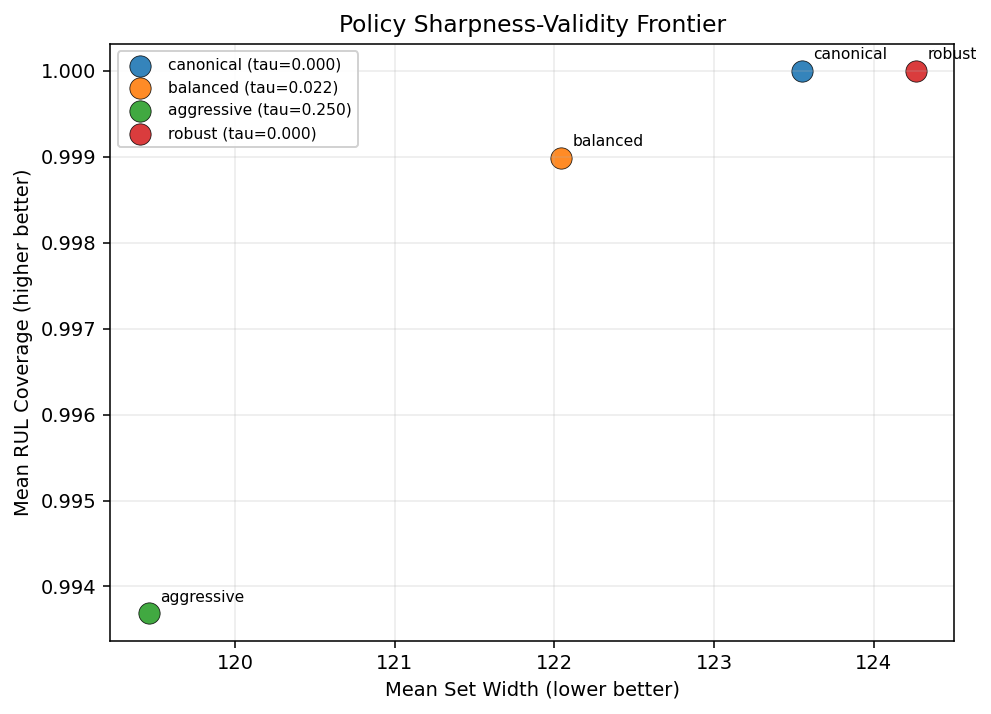
\includegraphics[width=0.62\textwidth]{figures/policy_sharpness_frontier.png}
\caption{Policy sharpness-validity frontier (mean set width vs mean coverage; legend includes tau max).}
\label{fig:policy-sharpness-frontier}
\end{figure}

\begin{figure}[t]
\centering
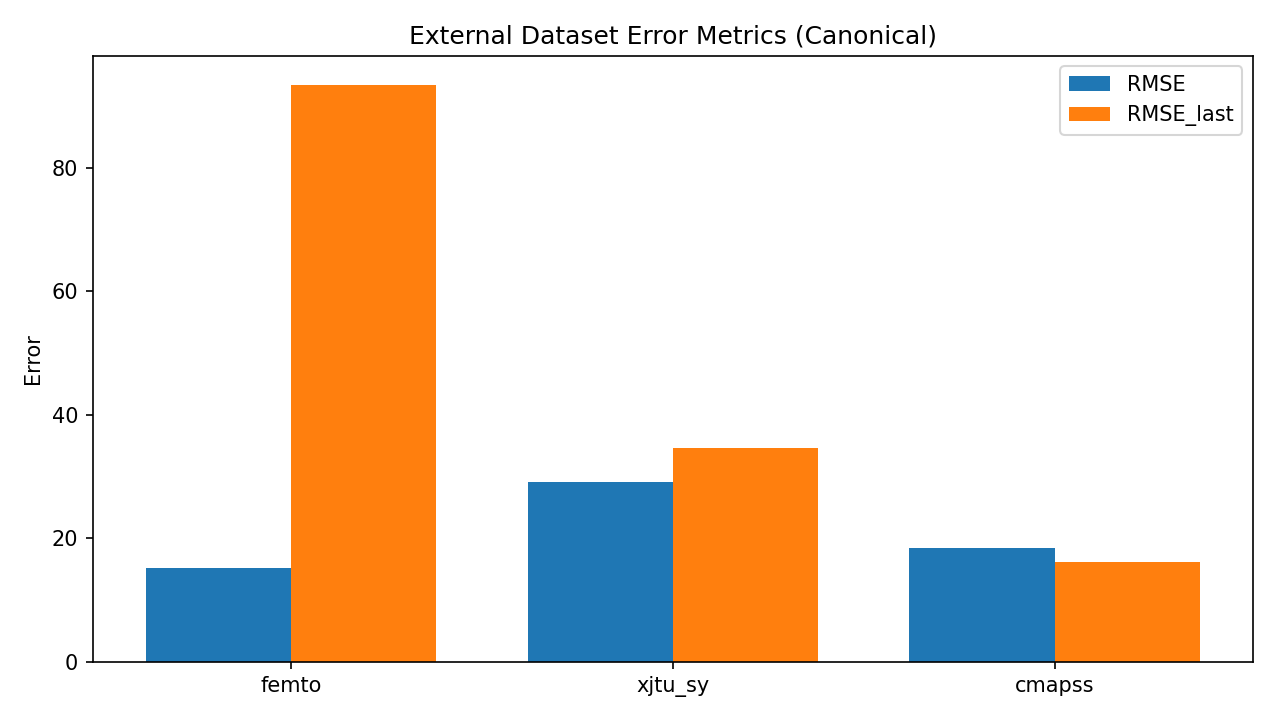
\includegraphics[width=0.48\textwidth]{figures/external_metrics_overview.png}\hfill
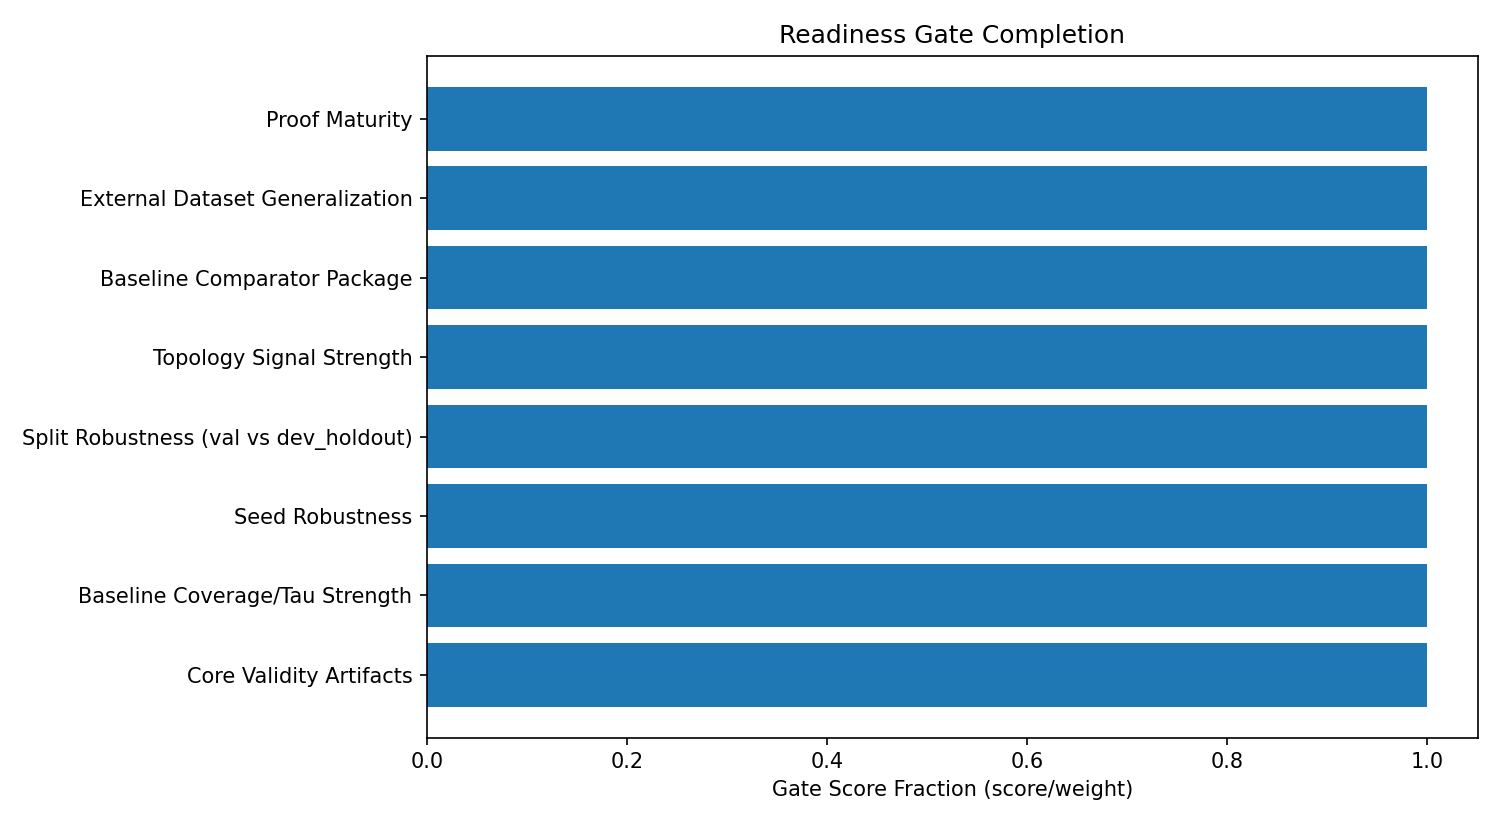
\includegraphics[width=0.48\textwidth]{figures/readiness_gates.png}
\caption{Canonical external errors and readiness gate completion.}
\label{fig:canonical-summary}
\end{figure}

\begin{figure}[t]
\centering

\includegraphics[width=0.32\textwidth]{figures/topology_vs_rul_bins.png}\hfill

\includegraphics[width=0.32\textwidth]{figures/surface_h1_vs_rul_coverage.png}\hfill

\includegraphics[width=0.32\textwidth]{figures/gamma_vs_pred_mae.png}
\caption{Topology-behavior diagnostics from canonical publication artifacts.}
\label{fig:topology-diags}
\end{figure}

\section{Reproducibility and Integrity}
The manuscript build is coupled to automated checks:
\begin{itemize}[leftmargin=1.3em]
\item gate summary: \url{outputs/publication_full_rtx4050/publication_gate_summary.json};
\item paper honesty report: \url{outputs/publication_full_rtx4050/paper_release/reports/paper_honesty_report.json};
\item suspicious-values audit: \url{outputs/publication_full_rtx4050/phd_suspicious_values_audit.json};
\item generated table provenance: \url{paper/generated/provenance.json}.
\end{itemize}
No metric in the canonical snapshot is manually edited; all are read directly from JSON artifacts.

\section{Limitations}
\begin{itemize}[leftmargin=1.3em]
\item Even after promoting a sharper gate-clearing external policy, width contraction remains uneven: XJTU-SY stays near the \num{125}-step support and the sweep-optimal point on C-MAPSS sits close to the tau target, so the canonical package must remain slightly more conservative than the frontier optimum.
\item Replay frontier granularity is still moderate; a denser grid could map the Pareto boundary more precisely.
\item Broader true retrain coverage now reaches FEMTO, XJTU-SY, and C-MAPSS, and the retrained replay sweep identifies target-valid sharper points down to mean width \num{118.0}; however, the sharpest point that also clears the stricter external gate is more conservative.
\item External sample size is limited on the smallest datasets, with only 4 FEMTO test runs and 2 XJTU-SY test runs in the current artifact-locked package.
\item Internal readiness score is not a substitute for independent external review.
\end{itemize}

\section{Conclusion}
The package is audit-ready and manuscript-compilable with artifact-locked results and explicit risk disclosures. Canonical external claims are reproducible and pass integrity checks. Remaining publication risk is primarily reviewer-facing: dataset-dependent external sharpness (especially XJTU-SY near-full width), limited external run counts on FEMTO/XJTU-SY, and the narrow gap between the replay frontier optimum and the stricter gate-clearing canonical point rather than artifact inconsistency.

\bibliographystyle{plainnat}
\bibliography{references}

\end{document}
